\subsection{Segmentation}
\subsubsection{Felzenszwalb's method}
\begin{figure}[htb!]
\centering
\begin{subfigure}{.3\textwidth}

\includegraphics[width=\textwidth]{images/rufy_d.png}
\caption{Before preprocessing.}
\end{subfigure}
\begin{subfigure}{.3\textwidth}
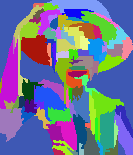
\includegraphics[width=\textwidth]{images/luffyK100.png}
\caption{With $k = 100$.}
\label{fig:smallKSegmentation}
\end{subfigure}
\begin{subfigure}{.3\textwidth}
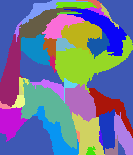
\includegraphics[width=\textwidth]{images/luffyK1000.png}
\caption{With $k = 1000$.}
\label{fig:largeKSegmentation}
\end{subfigure}
\caption{Segmentation results with Felzenszwalb's method, with a small $k$ and a larger $k$.}
\end{figure}

The segmentation method by P. F. Felzenszwalb and D. P. Huttenlocher, described in detail in \cite{felzenszwalb2004efficient}, is an efficient graph-based segmentation method for color images.

\paragraph{The method} Let $I$ be a color image. The algorithm considers a graph $G = (V,E)$ defined on the set of pixels of $I$ with weight function $w$ measuring dissimilarity between pixels. Let $n$ be the number of vertices and $m$ the number of edges of $G$. The pseudo code of the algorithm is given in algorithm \autoref{alg:felzenszwalb}, where $MInt : S \times S \rightarrow \mathbb{R}^+$ for some segmentation $S$ is defined by:
\[
MInt(C_1, C_2) = \min(Int(C_1) + \tau(C_1), Int(C_2) + \tau(C_2))
\]
$\tau(C) = \frac{k}{|C|}$ is a threshold function for a scale parameter $k$, and $Int(C)$ measure the internal difference of a component $C$, defined by
the largest weight of the minimum spanning tree of $C$:
\[
Int(C) = \max_{\{u,v\} \in MST(C, E)} w(u,v)
\]

\begin{algorithm}
\caption{Felzenszwalb's segmentation algorithm}
\label{alg:felzenszwalb}

\begin{algorithmic}[1]
\Function{Felzenszwalb}{$G = (V, E)$}
\State Sort $E$ into $\pi = (o_1, ..., o_m)$ by ascending edge weights
\State Initialize $S_0$ with each vertex in its own component
\For{$q \gets 1$ to $m$}
\State Let $\{u,v\} = o_q$ the $q^{th}$ edge in the ordering
\State Let $C_u$ and $C_v$ the components containing $u$ and $v$ in $S_{q-1}$
\If{$C_u \neq C_v$ and $w(u,v) \leq MInt(C_u, C_v)$}
\State $S_q$ is obtained by merging $C_u$ and $C_v$ in $S_{q-1}$
\Else
\State $S_q$ is just $S_{q-1}$
\EndIf
\EndFor
\Return $S_m$
\EndFunction
\end{algorithmic}
\end{algorithm}

\paragraph{Theoretical justification} The authors show that this algorithm results in a segmentation which is neither too coarse nor too fine, according to a precise notion of boundary between segments. This is interesting for animation character images, which are characterized by large areas of homogeneous color, which this algorithm capture reasonably well.

\paragraph{Implementation} The algorithm can be implemented to run very efficiently. Using a disjoint set forest data structure for the segmentation allows determining the component of a vertex and merging components to be performed in amortized $O(\alpha(n))$ time where $\alpha$ is the inverse of the Ackermann function. Computing $MInt$ between each iteration can be done in constant $O(1)$ time. With an adjacency list data structure for the graph $G$, it is easy to list all edges in $O(m)$ time. This makes clear that the time behavior of the algorithm is dominated by the initial sorting of edges, which can be computed in $O(m\log(m))$ time using an optimal comparison sort like merge sort.

The authors study the case where $G$ is an $8$-connected graph and where it is a variation on the $K$-nearest-neighbor graph\footnotemark
\footnotetext{
While a non-mutual $K$-nearest neighbor graph is not necessarily sparse, the authors assert that it is in their paper. As their graph construction is also not made explicit in the paper, and their source code only include an $8$-connected graph, we proceed under the optimistic assumption that the authors use a variation on the $K$-nearest-neighbor graph which is actually sparse.
}
 in $(x, y, r, g, b)$ feature space. Since both classes of graphs are sparse - the number of edges is within a constant factor of the number of vertices - this makes the time complexity of the algorithm $O(n\log(n))$.

\paragraph{Results and analysis} Although this algorithm is efficient, it suffers from a few drawbacks. The method as described above tends to create many very small components, which can be solved by a post-processing step greedily merging components smaller than a threshold. It also tends to produce segments of similar size, which in the case of animation character image is not desirable. It produces either an oversegmentation where large segments are separated in many small ones (\autoref{fig:smallKSegmentation}), or an undersegmentation where smaller segments are incorrectly merged into larger ones (\autoref{fig:largeKSegmentation}). To solve this issue, we introduced a post-processing step which we present in the next section (\autoref{sec:hueMerging}).

\subsubsection{Hue-based segment merging}
\label{sec:hueMerging}

Felzenszwalb's method, using a small enough scale parameter, tends to produce over segmentations of the image (relevant areas in the image are divided in multiple segments), with segments of similar area. Furthermore, using a $4$-connected graph, it cannot produce spatially disconnected segments, although such cases arise due to changes in posture or occlusion by other objects. To solve this issue, we introduced a post-processing step merging segments whose average hue are "close enough" in some sense, to produce a suitable segmentation with varying segment sizes and disconnected segments.

\paragraph{The method} We consider a segmentation $S$ for a color image $I$, our algorithm outputs a new segmentation for $I$. It proceeds by considering the complete graph on the set of segments of the image, with edges weighted by absolute hue difference. We then consider a small fraction of these edges in ascending order of weight, and fuse the corresponding segments. The pseudo code of the algorithm is given in algorithm \autoref{alg:hueMerging}.

\begin{algorithm}
\caption{Hue-base segment merging algorithm}
\label{alg:hueMerging}

\begin{algorithmic}[1]
\Function{HueMerging}{$I$, $S = \{S_1, ..., S_q\}$, $k \in \mathbb{N} - \{0\}$}
\State $E \gets \emptyset$
\For{each unordered pair $\{S_i, S_j\}$ in $S$}
\State Let $h_i$ and $h_j$ the average hue of $S_i$ and $S_j$ in $I$ respectively.
\State $E \gets E \cup \{(i, j, |h_i - h_j| )\}$
\EndFor
\For{$i \gets 1$ to $\lfloor \frac{q}{k} \rfloor$}
\State Remove edge $(i,j,w)$ with smallest weight $w$ from $E$.
\State Merge segments containing $S_i$ and $S_j$ in $S$.
\EndFor
\Return $S$
\EndFunction
\end{algorithmic}
\end{algorithm}

\paragraph{Theoretical justification} This is mostly a heuristic method which relies on greedy assumptions for efficiency. For instance we assume that the difference in average hue between the merged segment is small enough that the average hue of the new segment does not need recomputing. As we merge them from smallest hue difference to largest, this assumption holds to some extent. Although computing the new hue can be done efficiently by associativity of the barycenter, it would require resorting the data structure for $E$ to account for the changes - which propagate inside the graph in a non-trivial way.

\paragraph{Implementation} Computing the average hue for each segment can be done in $O(n\alpha(n))$ steps using a disjoint set forest data structure for $S$ where $\alpha$ is the inverse of the Ackermann function and $n$ is the number of pixels in the image - assuming the hue of each pixels was precomputed as part of a preprocessing step. Using a binary heap data structure for $E$ makes computing the edges weight run in $O(q^2)$ time, and the second loop then runs in $O(\lfloor \frac{q}{k} \rfloor \log(q))$. As there is, to the author's knowledge, no direct relationship between $q$ and $n$ (besides $q \leq n$) allowing us to decide which of the first $2$ steps dominates the author, we will leave the overall time complexity as $O(n\alpha(n) + q^2)$.

\paragraph{Results and analysis} As a post-processing step to Felzenszwalb's method, this algorithm gives segmentation which solves the issues mentioned earlier - segments of varying size, connecting areas which are spatially disconnected. This yields segmentation which correspond better to human perception, and are overall more consistent across images of the same character, which is essential to classification.